\documentclass[twoside]{book}

% Packages required by doxygen
\usepackage{calc}
\usepackage{doxygen}
\usepackage{graphicx}
\usepackage[utf8]{inputenc}
\usepackage{makeidx}
\usepackage{multicol}
\usepackage{multirow}
\usepackage{textcomp}
\usepackage[table]{xcolor}

% Font selection
\usepackage[T1]{fontenc}
\usepackage{mathptmx}
\usepackage[scaled=.90]{helvet}
\usepackage{courier}
\usepackage{amssymb}
\usepackage{sectsty}
\renewcommand{\familydefault}{\sfdefault}
\allsectionsfont{%
  \fontseries{bc}\selectfont%
  \color{darkgray}%
}
\renewcommand{\DoxyLabelFont}{%
  \fontseries{bc}\selectfont%
  \color{darkgray}%
}

% Page & text layout
\usepackage{geometry}
\geometry{%
  a4paper,%
  top=2.5cm,%
  bottom=2.5cm,%
  left=2.5cm,%
  right=2.5cm%
}
\tolerance=750
\hfuzz=15pt
\hbadness=750
\setlength{\emergencystretch}{15pt}
\setlength{\parindent}{0cm}
\setlength{\parskip}{0.2cm}
\makeatletter
\renewcommand{\paragraph}{%
  \@startsection{paragraph}{4}{0ex}{-1.0ex}{1.0ex}{%
    \normalfont\normalsize\bfseries\SS@parafont%
  }%
}
\renewcommand{\subparagraph}{%
  \@startsection{subparagraph}{5}{0ex}{-1.0ex}{1.0ex}{%
    \normalfont\normalsize\bfseries\SS@subparafont%
  }%
}
\makeatother

% Headers & footers
\usepackage{fancyhdr}
\pagestyle{fancyplain}
\fancyhead[LE]{\fancyplain{}{\bfseries\thepage}}
\fancyhead[CE]{\fancyplain{}{}}
\fancyhead[RE]{\fancyplain{}{\bfseries\leftmark}}
\fancyhead[LO]{\fancyplain{}{\bfseries\rightmark}}
\fancyhead[CO]{\fancyplain{}{}}
\fancyhead[RO]{\fancyplain{}{\bfseries\thepage}}
\fancyfoot[LE]{\fancyplain{}{}}
\fancyfoot[CE]{\fancyplain{}{}}
\fancyfoot[RE]{\fancyplain{}{\bfseries\scriptsize Generated on Mon Feb 1 2016 14\-:24\-:44 for Library\-Lib\-Lidar\-Lms151 by Doxygen }}
\fancyfoot[LO]{\fancyplain{}{\bfseries\scriptsize Generated on Mon Feb 1 2016 14\-:24\-:44 for Library\-Lib\-Lidar\-Lms151 by Doxygen }}
\fancyfoot[CO]{\fancyplain{}{}}
\fancyfoot[RO]{\fancyplain{}{}}
\renewcommand{\footrulewidth}{0.4pt}
\renewcommand{\chaptermark}[1]{%
  \markboth{#1}{}%
}
\renewcommand{\sectionmark}[1]{%
  \markright{\thesection\ #1}%
}

% Indices & bibliography
\usepackage{natbib}
\usepackage[titles]{tocloft}
\setcounter{tocdepth}{3}
\setcounter{secnumdepth}{5}
\makeindex

% Hyperlinks (required, but should be loaded last)
\usepackage{ifpdf}
\ifpdf
  \usepackage[pdftex,pagebackref=true]{hyperref}
\else
  \usepackage[ps2pdf,pagebackref=true]{hyperref}
\fi
\hypersetup{%
  colorlinks=true,%
  linkcolor=blue,%
  citecolor=blue,%
  unicode%
}

% Custom commands
\newcommand{\clearemptydoublepage}{%
  \newpage{\pagestyle{empty}\cleardoublepage}%
}


%===== C O N T E N T S =====

\begin{document}

% Titlepage & ToC
\hypersetup{pageanchor=false}
\pagenumbering{roman}
\begin{titlepage}
\vspace*{7cm}
\begin{center}%
{\Large Library\-Lib\-Lidar\-Lms151 }\\
\vspace*{1cm}
{\large Generated by Doxygen 1.8.6}\\
\vspace*{0.5cm}
{\small Mon Feb 1 2016 14:24:44}\\
\end{center}
\end{titlepage}
\clearemptydoublepage
\tableofcontents
\clearemptydoublepage
\pagenumbering{arabic}
\hypersetup{pageanchor=true}

%--- Begin generated contents ---
\chapter{File Index}
\section{File List}
Here is a list of all documented files with brief descriptions\-:\begin{DoxyCompactList}
\item\contentsline{section}{\hyperlink{Driver__TcpSocketDriver_8c}{Driver\-\_\-\-Tcp\-Socket\-Driver.\-c} \\*Source file of Tcp\-Socket\-Driver Service }{\pageref{Driver__TcpSocketDriver_8c}}{}
\end{DoxyCompactList}

\chapter{File Documentation}
\hypertarget{Library__LibLidarLms151_8c}{\section{Library\-\_\-\-Lib\-Lidar\-Lms151.\-c File Reference}
\label{Library__LibLidarLms151_8c}\index{Library\-\_\-\-Lib\-Lidar\-Lms151.\-c@{Library\-\_\-\-Lib\-Lidar\-Lms151.\-c}}
}


Fichier Source du Service Lib\-Lidar\-Lms151.  


{\ttfamily \#include \char`\"{}types.\-h\char`\"{}}\\*
{\ttfamily \#include \char`\"{}Library\-\_\-\-Std\-Lib.\-h\char`\"{}}\\*
{\ttfamily \#include \char`\"{}Library\-\_\-\-Lib\-Lidar\-Lms151.\-h\char`\"{}}\\*
{\ttfamily \#include \char`\"{}Driver\-\_\-\-Tcp\-Socket\-Driver.\-h\char`\"{}}\\*
{\ttfamily \#include $<$string.\-h$>$}\\*
{\ttfamily \#include $<$stdlib.\-h$>$}\\*
{\ttfamily \#include $<$stdio.\-h$>$}\\*
{\ttfamily \#include $<$errno.\-h$>$}\\*
Include dependency graph for Library\-\_\-\-Lib\-Lidar\-Lms151.\-c\-:
\nopagebreak
\begin{figure}[H]
\begin{center}
\leavevmode
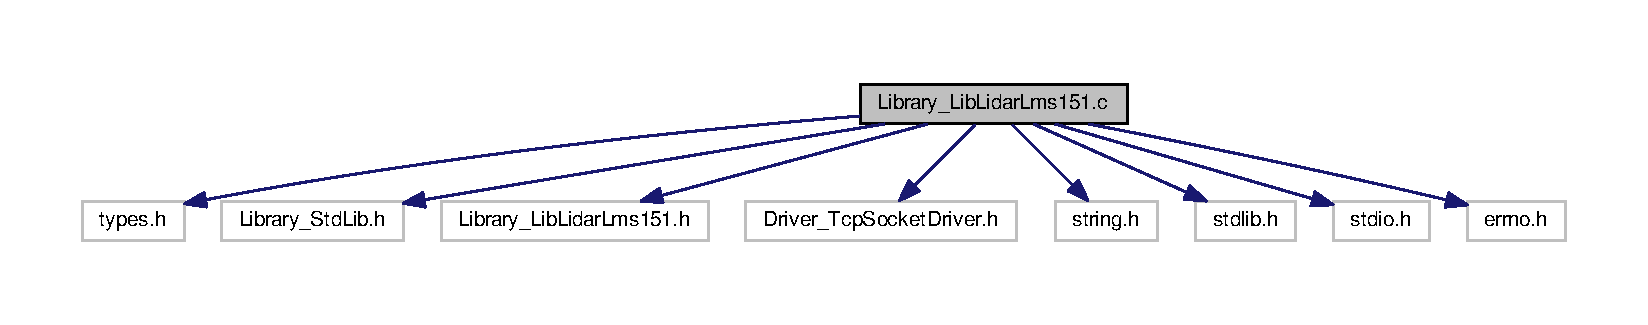
\includegraphics[width=350pt]{Library__LibLidarLms151_8c__incl}
\end{center}
\end{figure}
\subsection*{Macros}
\begin{DoxyCompactItemize}
\item 
\#define \hyperlink{Library__LibLidarLms151_8c_aa37fd732d743e2ab7528ed209edb3dfa}{K\-\_\-\-B\-U\-F\-F\-E\-R\-\_\-\-S\-I\-Z\-E\-\_\-\-M\-A\-X}~262144ul				/$\ast$! buffer maximal size value $\ast$/
\item 
\hypertarget{Library__LibLidarLms151_8c_aa796a946499ef71ebd208d87300b07f0}{\#define {\bfseries K\-\_\-\-S\-T\-A\-R\-T}~1						/$\ast$! Start value $\ast$/}\label{Library__LibLidarLms151_8c_aa796a946499ef71ebd208d87300b07f0}

\item 
\hypertarget{Library__LibLidarLms151_8c_a869034147b9dd5df11bd4234e5ca7ce8}{\#define {\bfseries K\-\_\-\-A\-M\-O\-U\-N\-T\-\_\-\-O\-F\-\_\-\-E\-N\-C\-O\-D\-E\-R\-S\-\_\-\-M\-A\-X}~3						/$\ast$! Maximum amount of encoders $\ast$/}\label{Library__LibLidarLms151_8c_a869034147b9dd5df11bd4234e5ca7ce8}

\item 
\hypertarget{Library__LibLidarLms151_8c_a33e3d0b43eae746eb5ab1b18acede2d6}{\#define {\bfseries K\-\_\-\-A\-M\-O\-U\-N\-T\-\_\-\-O\-F\-\_\-16\-B\-I\-T\-S\-\_\-\-C\-H\-A\-N\-N\-E\-L\-S\-\_\-\-M\-A\-X}~2						/$\ast$! Maximum amount of 16bits channels $\ast$/}\label{Library__LibLidarLms151_8c_a33e3d0b43eae746eb5ab1b18acede2d6}

\item 
\hypertarget{Library__LibLidarLms151_8c_aeb4035cfa542a92d07f083b79d17ad36}{\#define {\bfseries K\-\_\-\-A\-M\-O\-U\-N\-T\-\_\-\-O\-F\-\_\-8\-B\-I\-T\-S\-\_\-\-C\-H\-A\-N\-N\-E\-L\-S\-\_\-\-M\-A\-X}~2						/$\ast$! Maximum amount of 8bits channels $\ast$/}\label{Library__LibLidarLms151_8c_aeb4035cfa542a92d07f083b79d17ad36}

\end{DoxyCompactItemize}
\subsection*{Enumerations}
\begin{DoxyCompactItemize}
\item 
enum \hyperlink{Library__LibLidarLms151_8c_ae35bebf116d718afd22cc5652c5a30c1}{te\-\_\-command\-\_\-status} \{ {\bfseries E\-\_\-\-C\-O\-M\-M\-A\-N\-D\-\_\-\-E\-R\-R\-O\-R} =0, 
{\bfseries E\-\_\-\-C\-O\-M\-M\-A\-N\-D\-\_\-\-S\-U\-C\-C\-E\-S\-S}
 \}
\begin{DoxyCompactList}\small\item\em define the command status \end{DoxyCompactList}\item 
enum \hyperlink{Library__LibLidarLms151_8c_a599a5afb785ebdf3627653441ec4068f}{te\-\_\-start\-\_\-status} \{ {\bfseries E\-\_\-\-S\-T\-A\-R\-T\-\_\-\-N\-O\-\_\-\-E\-R\-R\-O\-R} =0, 
{\bfseries E\-\_\-\-S\-T\-A\-R\-T\-\_\-\-N\-O\-T\-\_\-\-A\-L\-L\-O\-W\-E\-D}
 \}
\begin{DoxyCompactList}\small\item\em define the start status \end{DoxyCompactList}\item 
enum \hyperlink{Library__LibLidarLms151_8c_a51a75b37643898bb45705246e5225eac}{te\-\_\-sub\-State} \{ {\bfseries E\-\_\-\-I\-D\-L\-E} = 0, 
\hyperlink{Library__LibLidarLms151_8c_a51a75b37643898bb45705246e5225eaca709ccc7c35719235536104906d05b0c5}{E\-\_\-\-R\-E\-A\-D}, 
\hyperlink{Library__LibLidarLms151_8c_a51a75b37643898bb45705246e5225eaca7b7d81ed853af64388be3a5e5b371eae}{E\-\_\-\-E\-R\-R\-O\-R}
 \}
\begin{DoxyCompactList}\small\item\em define the mode substate \end{DoxyCompactList}\item 
enum \hyperlink{Library__LibLidarLms151_8c_ae46cfb453101b61ff4f5f1ef5b14ff64}{te\-\_\-\-Read\-Status} \{ {\bfseries E\-\_\-\-R\-E\-A\-D\-\_\-\-B\-U\-S\-Y} =0, 
\hyperlink{Library__LibLidarLms151_8c_ae46cfb453101b61ff4f5f1ef5b14ff64a9d33570b5ccf5a1891cdf5191ac59a06}{E\-\_\-\-R\-E\-A\-D\-\_\-\-F\-I\-N\-I\-S\-H}, 
\hyperlink{Library__LibLidarLms151_8c_ae46cfb453101b61ff4f5f1ef5b14ff64a310c58933b364054ebe85d0e68239c3d}{E\-\_\-\-R\-E\-A\-D\-\_\-\-N\-O\-\_\-\-D\-A\-T\-A}
 \}
\begin{DoxyCompactList}\small\item\em define the read status \end{DoxyCompactList}\item 
enum \hyperlink{Library__LibLidarLms151_8c_a9625f39a001943d19e2475eb080ac32b}{te\-\_\-\-Content\-Out\-Channel} \{ {\bfseries E\-\_\-\-O\-U\-T\-\_\-\-D\-I\-S\-T1} = 0, 
\hyperlink{Library__LibLidarLms151_8c_a9625f39a001943d19e2475eb080ac32ba849130bdeb0ec2daf7a4bc36f127d99e}{E\-\_\-\-O\-U\-T\-\_\-\-D\-I\-S\-T2}, 
\hyperlink{Library__LibLidarLms151_8c_a9625f39a001943d19e2475eb080ac32ba6d14f9ccb0d2ff73781863a0d266c39a}{E\-\_\-\-O\-U\-T\-\_\-\-R\-S\-S\-I1}, 
\hyperlink{Library__LibLidarLms151_8c_a9625f39a001943d19e2475eb080ac32ba7a6db760c9baa9d4e5afd0594da666b3}{E\-\_\-\-O\-U\-T\-\_\-\-R\-S\-S\-I2}
 \}
\begin{DoxyCompactList}\small\item\em define the lidar Content Out channel \end{DoxyCompactList}\end{DoxyCompactItemize}
\subsection*{Functions}
\begin{DoxyCompactItemize}
\item 
Std\-\_\-\-Return\-Type \hyperlink{Library__LibLidarLms151_8c_a7b9683e9173da5acc00d3163420f1641}{Lib\-Lidar\-Lms151\-\_\-\-Initialize} (void)
\begin{DoxyCompactList}\small\item\em this function initialize module \end{DoxyCompactList}\item 
Std\-\_\-\-Return\-Type \hyperlink{Library__LibLidarLms151_8c_a5529e161afb1cc77407a08342c65eab2}{Lib\-Lidar\-Lms151\-\_\-\-Configure} (const ts\-\_\-\-Lib\-Lidar\-Lms151\-\_\-\-Configuration $\ast$const ps\-\_\-\-Lib\-Lidar\-Lms151\-\_\-\-Configuration)
\item 
Std\-\_\-\-Return\-Type \hyperlink{Library__LibLidarLms151_8c_a1ec6c5af5244dc78c11e4bedc8cb62bf}{Lib\-Lidar\-Lms151\-\_\-\-Manage} (void)
\begin{DoxyCompactList}\small\item\em this function is the central point of the library, it manage the laser \end{DoxyCompactList}\item 
Std\-\_\-\-Return\-Type \hyperlink{Library__LibLidarLms151_8c_a4693c1cfe2e441d7161921c091715f27}{Lib\-Lidar\-Lms151\-\_\-\-Open} (void)
\begin{DoxyCompactList}\small\item\em this function will open Tcp Socket needed for communication with Lms151 \end{DoxyCompactList}\item 
Std\-\_\-\-Return\-Type \hyperlink{Library__LibLidarLms151_8c_a8eba74dac1063ab5a3859510566921f2}{Lib\-Lidar\-Lms151\-\_\-\-Close} (void)
\begin{DoxyCompactList}\small\item\em this function will close Tcp Socket needed for communication with Lms151 \end{DoxyCompactList}\item 
Std\-\_\-\-Return\-Type \hyperlink{Library__LibLidarLms151_8c_a6e4c234961f05d70298a4bb5c157fe5c}{Lib\-Lidar\-Lms151\-\_\-\-Get\-\_\-\-Timestamp} (uint32 $\ast$const pu32\-\_\-\-Timestamp)
\begin{DoxyCompactList}\small\item\em this function will return Laser data Timestamp \end{DoxyCompactList}\item 
Std\-\_\-\-Return\-Type \hyperlink{Library__LibLidarLms151_8c_a9efbf9532dae8a4f3304d7cb6eed78d1}{Lib\-Lidar\-Lms151\-\_\-\-Get\-\_\-\-Scan} (ts\-\_\-\-Lib\-Lidar\-Lms151\-\_\-scan\-\_\-data $\ast$const ps\-\_\-\-Lib\-Lidar\-Lms151\-\_\-scan\-\_\-data)
\begin{DoxyCompactList}\small\item\em this function will return scan values \end{DoxyCompactList}\item 
Std\-\_\-\-Return\-Type \hyperlink{Library__LibLidarLms151_8c_a0c8651f8a7b6549aecaecae2ee5518ea}{Lib\-Lidar\-Lms151\-\_\-\-Get\-\_\-\-Internal\-State} (te\-\_\-\-Internal\-State\-Machine $\ast$const pe\-\_\-\-State)
\begin{DoxyCompactList}\small\item\em this function will return internal state \end{DoxyCompactList}\item 
Std\-\_\-\-Return\-Type \hyperlink{Library__LibLidarLms151_8c_a89b93dbf0565748d08406a15a075263b}{Lib\-Lidar\-Lms151\-\_\-\-Get\-\_\-\-Status} (te\-\_\-\-Lib\-Lidar\-Lms151\-\_\-device\-\_\-status $\ast$const pe\-\_\-\-Lib\-Lidar\-Lms151\-\_\-device\-\_\-status)
\begin{DoxyCompactList}\small\item\em this function will return laser status \end{DoxyCompactList}\item 
Std\-\_\-\-Return\-Type \hyperlink{Library__LibLidarLms151_8c_aa419ecd7693e2c184d1195a4b2f96d91}{Lib\-Lidar\-Lms151\-\_\-\-Get\-\_\-\-Mode} (te\-\_\-mode $\ast$const pe\-\_\-\-Mode)
\begin{DoxyCompactList}\small\item\em this function will return global mode \end{DoxyCompactList}\end{DoxyCompactItemize}


\subsection{Detailed Description}
Fichier Source du Service Lib\-Lidar\-Lms151. \$\-Source\-: \hyperlink{Library__LibLidarLms151_8c}{Library\-\_\-\-Lib\-Lidar\-Lms151.\-c} \$\-Author\-: Slo \$\-Date\-: 2016/01/14 

\subsection{Macro Definition Documentation}
\hypertarget{Library__LibLidarLms151_8c_aa37fd732d743e2ab7528ed209edb3dfa}{\index{Library\-\_\-\-Lib\-Lidar\-Lms151.\-c@{Library\-\_\-\-Lib\-Lidar\-Lms151.\-c}!K\-\_\-\-B\-U\-F\-F\-E\-R\-\_\-\-S\-I\-Z\-E\-\_\-\-M\-A\-X@{K\-\_\-\-B\-U\-F\-F\-E\-R\-\_\-\-S\-I\-Z\-E\-\_\-\-M\-A\-X}}
\index{K\-\_\-\-B\-U\-F\-F\-E\-R\-\_\-\-S\-I\-Z\-E\-\_\-\-M\-A\-X@{K\-\_\-\-B\-U\-F\-F\-E\-R\-\_\-\-S\-I\-Z\-E\-\_\-\-M\-A\-X}!Library_LibLidarLms151.c@{Library\-\_\-\-Lib\-Lidar\-Lms151.\-c}}
\subsubsection[{K\-\_\-\-B\-U\-F\-F\-E\-R\-\_\-\-S\-I\-Z\-E\-\_\-\-M\-A\-X}]{\setlength{\rightskip}{0pt plus 5cm}\#define K\-\_\-\-B\-U\-F\-F\-E\-R\-\_\-\-S\-I\-Z\-E\-\_\-\-M\-A\-X~262144ul				/$\ast$! buffer maximal size value $\ast$/}}\label{Library__LibLidarLms151_8c_aa37fd732d743e2ab7528ed209edb3dfa}
Global constant Reserved value \char`\"{}1\char`\"{} 

\subsection{Enumeration Type Documentation}
\hypertarget{Library__LibLidarLms151_8c_a9625f39a001943d19e2475eb080ac32b}{\index{Library\-\_\-\-Lib\-Lidar\-Lms151.\-c@{Library\-\_\-\-Lib\-Lidar\-Lms151.\-c}!te\-\_\-\-Content\-Out\-Channel@{te\-\_\-\-Content\-Out\-Channel}}
\index{te\-\_\-\-Content\-Out\-Channel@{te\-\_\-\-Content\-Out\-Channel}!Library_LibLidarLms151.c@{Library\-\_\-\-Lib\-Lidar\-Lms151.\-c}}
\subsubsection[{te\-\_\-\-Content\-Out\-Channel}]{\setlength{\rightskip}{0pt plus 5cm}enum {\bf te\-\_\-\-Content\-Out\-Channel}}}\label{Library__LibLidarLms151_8c_a9625f39a001943d19e2475eb080ac32b}


define the lidar Content Out channel 

\begin{Desc}
\item[Enumerator]\par
\begin{description}
\index{E\-\_\-\-O\-U\-T\-\_\-\-D\-I\-S\-T2@{E\-\_\-\-O\-U\-T\-\_\-\-D\-I\-S\-T2}!Library\-\_\-\-Lib\-Lidar\-Lms151.\-c@{Library\-\_\-\-Lib\-Lidar\-Lms151.\-c}}\index{Library\-\_\-\-Lib\-Lidar\-Lms151.\-c@{Library\-\_\-\-Lib\-Lidar\-Lms151.\-c}!E\-\_\-\-O\-U\-T\-\_\-\-D\-I\-S\-T2@{E\-\_\-\-O\-U\-T\-\_\-\-D\-I\-S\-T2}}\item[{\em 
\hypertarget{Library__LibLidarLms151_8c_a9625f39a001943d19e2475eb080ac32ba849130bdeb0ec2daf7a4bc36f127d99e}{E\-\_\-\-O\-U\-T\-\_\-\-D\-I\-S\-T2}\label{Library__LibLidarLms151_8c_a9625f39a001943d19e2475eb080ac32ba849130bdeb0ec2daf7a4bc36f127d99e}
}]Content channel is D\-I\-S\-T1 \index{E\-\_\-\-O\-U\-T\-\_\-\-R\-S\-S\-I1@{E\-\_\-\-O\-U\-T\-\_\-\-R\-S\-S\-I1}!Library\-\_\-\-Lib\-Lidar\-Lms151.\-c@{Library\-\_\-\-Lib\-Lidar\-Lms151.\-c}}\index{Library\-\_\-\-Lib\-Lidar\-Lms151.\-c@{Library\-\_\-\-Lib\-Lidar\-Lms151.\-c}!E\-\_\-\-O\-U\-T\-\_\-\-R\-S\-S\-I1@{E\-\_\-\-O\-U\-T\-\_\-\-R\-S\-S\-I1}}\item[{\em 
\hypertarget{Library__LibLidarLms151_8c_a9625f39a001943d19e2475eb080ac32ba6d14f9ccb0d2ff73781863a0d266c39a}{E\-\_\-\-O\-U\-T\-\_\-\-R\-S\-S\-I1}\label{Library__LibLidarLms151_8c_a9625f39a001943d19e2475eb080ac32ba6d14f9ccb0d2ff73781863a0d266c39a}
}]Content channel is D\-I\-S\-T2 \index{E\-\_\-\-O\-U\-T\-\_\-\-R\-S\-S\-I2@{E\-\_\-\-O\-U\-T\-\_\-\-R\-S\-S\-I2}!Library\-\_\-\-Lib\-Lidar\-Lms151.\-c@{Library\-\_\-\-Lib\-Lidar\-Lms151.\-c}}\index{Library\-\_\-\-Lib\-Lidar\-Lms151.\-c@{Library\-\_\-\-Lib\-Lidar\-Lms151.\-c}!E\-\_\-\-O\-U\-T\-\_\-\-R\-S\-S\-I2@{E\-\_\-\-O\-U\-T\-\_\-\-R\-S\-S\-I2}}\item[{\em 
\hypertarget{Library__LibLidarLms151_8c_a9625f39a001943d19e2475eb080ac32ba7a6db760c9baa9d4e5afd0594da666b3}{E\-\_\-\-O\-U\-T\-\_\-\-R\-S\-S\-I2}\label{Library__LibLidarLms151_8c_a9625f39a001943d19e2475eb080ac32ba7a6db760c9baa9d4e5afd0594da666b3}
}]Content channel is R\-S\-S\-I1

Content channel is R\-S\-S\-I2 \end{description}
\end{Desc}
\hypertarget{Library__LibLidarLms151_8c_ae46cfb453101b61ff4f5f1ef5b14ff64}{\index{Library\-\_\-\-Lib\-Lidar\-Lms151.\-c@{Library\-\_\-\-Lib\-Lidar\-Lms151.\-c}!te\-\_\-\-Read\-Status@{te\-\_\-\-Read\-Status}}
\index{te\-\_\-\-Read\-Status@{te\-\_\-\-Read\-Status}!Library_LibLidarLms151.c@{Library\-\_\-\-Lib\-Lidar\-Lms151.\-c}}
\subsubsection[{te\-\_\-\-Read\-Status}]{\setlength{\rightskip}{0pt plus 5cm}enum {\bf te\-\_\-\-Read\-Status}}}\label{Library__LibLidarLms151_8c_ae46cfb453101b61ff4f5f1ef5b14ff64}


define the read status 

\begin{Desc}
\item[Enumerator]\par
\begin{description}
\index{E\-\_\-\-R\-E\-A\-D\-\_\-\-F\-I\-N\-I\-S\-H@{E\-\_\-\-R\-E\-A\-D\-\_\-\-F\-I\-N\-I\-S\-H}!Library\-\_\-\-Lib\-Lidar\-Lms151.\-c@{Library\-\_\-\-Lib\-Lidar\-Lms151.\-c}}\index{Library\-\_\-\-Lib\-Lidar\-Lms151.\-c@{Library\-\_\-\-Lib\-Lidar\-Lms151.\-c}!E\-\_\-\-R\-E\-A\-D\-\_\-\-F\-I\-N\-I\-S\-H@{E\-\_\-\-R\-E\-A\-D\-\_\-\-F\-I\-N\-I\-S\-H}}\item[{\em 
\hypertarget{Library__LibLidarLms151_8c_ae46cfb453101b61ff4f5f1ef5b14ff64a9d33570b5ccf5a1891cdf5191ac59a06}{E\-\_\-\-R\-E\-A\-D\-\_\-\-F\-I\-N\-I\-S\-H}\label{Library__LibLidarLms151_8c_ae46cfb453101b61ff4f5f1ef5b14ff64a9d33570b5ccf5a1891cdf5191ac59a06}
}]Read busy \index{E\-\_\-\-R\-E\-A\-D\-\_\-\-N\-O\-\_\-\-D\-A\-T\-A@{E\-\_\-\-R\-E\-A\-D\-\_\-\-N\-O\-\_\-\-D\-A\-T\-A}!Library\-\_\-\-Lib\-Lidar\-Lms151.\-c@{Library\-\_\-\-Lib\-Lidar\-Lms151.\-c}}\index{Library\-\_\-\-Lib\-Lidar\-Lms151.\-c@{Library\-\_\-\-Lib\-Lidar\-Lms151.\-c}!E\-\_\-\-R\-E\-A\-D\-\_\-\-N\-O\-\_\-\-D\-A\-T\-A@{E\-\_\-\-R\-E\-A\-D\-\_\-\-N\-O\-\_\-\-D\-A\-T\-A}}\item[{\em 
\hypertarget{Library__LibLidarLms151_8c_ae46cfb453101b61ff4f5f1ef5b14ff64a310c58933b364054ebe85d0e68239c3d}{E\-\_\-\-R\-E\-A\-D\-\_\-\-N\-O\-\_\-\-D\-A\-T\-A}\label{Library__LibLidarLms151_8c_ae46cfb453101b61ff4f5f1ef5b14ff64a310c58933b364054ebe85d0e68239c3d}
}]Read finished

No data read \end{description}
\end{Desc}
\hypertarget{Library__LibLidarLms151_8c_a51a75b37643898bb45705246e5225eac}{\index{Library\-\_\-\-Lib\-Lidar\-Lms151.\-c@{Library\-\_\-\-Lib\-Lidar\-Lms151.\-c}!te\-\_\-sub\-State@{te\-\_\-sub\-State}}
\index{te\-\_\-sub\-State@{te\-\_\-sub\-State}!Library_LibLidarLms151.c@{Library\-\_\-\-Lib\-Lidar\-Lms151.\-c}}
\subsubsection[{te\-\_\-sub\-State}]{\setlength{\rightskip}{0pt plus 5cm}enum {\bf te\-\_\-sub\-State}}}\label{Library__LibLidarLms151_8c_a51a75b37643898bb45705246e5225eac}


define the mode substate 

\begin{Desc}
\item[Enumerator]\par
\begin{description}
\index{E\-\_\-\-R\-E\-A\-D@{E\-\_\-\-R\-E\-A\-D}!Library\-\_\-\-Lib\-Lidar\-Lms151.\-c@{Library\-\_\-\-Lib\-Lidar\-Lms151.\-c}}\index{Library\-\_\-\-Lib\-Lidar\-Lms151.\-c@{Library\-\_\-\-Lib\-Lidar\-Lms151.\-c}!E\-\_\-\-R\-E\-A\-D@{E\-\_\-\-R\-E\-A\-D}}\item[{\em 
\hypertarget{Library__LibLidarLms151_8c_a51a75b37643898bb45705246e5225eaca709ccc7c35719235536104906d05b0c5}{E\-\_\-\-R\-E\-A\-D}\label{Library__LibLidarLms151_8c_a51a75b37643898bb45705246e5225eaca709ccc7c35719235536104906d05b0c5}
}]Mode is in I\-D\-L\-E state \index{E\-\_\-\-E\-R\-R\-O\-R@{E\-\_\-\-E\-R\-R\-O\-R}!Library\-\_\-\-Lib\-Lidar\-Lms151.\-c@{Library\-\_\-\-Lib\-Lidar\-Lms151.\-c}}\index{Library\-\_\-\-Lib\-Lidar\-Lms151.\-c@{Library\-\_\-\-Lib\-Lidar\-Lms151.\-c}!E\-\_\-\-E\-R\-R\-O\-R@{E\-\_\-\-E\-R\-R\-O\-R}}\item[{\em 
\hypertarget{Library__LibLidarLms151_8c_a51a75b37643898bb45705246e5225eaca7b7d81ed853af64388be3a5e5b371eae}{E\-\_\-\-E\-R\-R\-O\-R}\label{Library__LibLidarLms151_8c_a51a75b37643898bb45705246e5225eaca7b7d81ed853af64388be3a5e5b371eae}
}]Mode is actually in Read state

Mode is in Error state \end{description}
\end{Desc}


\subsection{Function Documentation}
\hypertarget{Library__LibLidarLms151_8c_a8eba74dac1063ab5a3859510566921f2}{\index{Library\-\_\-\-Lib\-Lidar\-Lms151.\-c@{Library\-\_\-\-Lib\-Lidar\-Lms151.\-c}!Lib\-Lidar\-Lms151\-\_\-\-Close@{Lib\-Lidar\-Lms151\-\_\-\-Close}}
\index{Lib\-Lidar\-Lms151\-\_\-\-Close@{Lib\-Lidar\-Lms151\-\_\-\-Close}!Library_LibLidarLms151.c@{Library\-\_\-\-Lib\-Lidar\-Lms151.\-c}}
\subsubsection[{Lib\-Lidar\-Lms151\-\_\-\-Close}]{\setlength{\rightskip}{0pt plus 5cm}Std\-\_\-\-Return\-Type Lib\-Lidar\-Lms151\-\_\-\-Close (
\begin{DoxyParamCaption}
\item[{void}]{}
\end{DoxyParamCaption}
)}}\label{Library__LibLidarLms151_8c_a8eba74dac1063ab5a3859510566921f2}


this function will close Tcp Socket needed for communication with Lms151 


\begin{DoxyParams}{Parameters}
{\em none} & \\
\hline
\end{DoxyParams}
\begin{DoxyReturn}{Returns}
Std\-\_\-\-Return\-Type \-:
\begin{DoxyItemize}
\item E\-\_\-\-N\-O\-T\-\_\-\-O\-K if module is not initialized or Tcp socket return an error
\item else E\-\_\-\-O\-K 
\end{DoxyItemize}
\end{DoxyReturn}
Tcp Socket Close Error, t\-\_\-\-Close\-\_\-\-Status is set to E\-\_\-\-N\-O\-T\-\_\-\-O\-K

no Tcp Socket Close Error, t\-\_\-\-Close\-\_\-\-Status is set to E\-\_\-\-O\-K

Module is not initialized, Halt \hypertarget{Library__LibLidarLms151_8c_a5529e161afb1cc77407a08342c65eab2}{\index{Library\-\_\-\-Lib\-Lidar\-Lms151.\-c@{Library\-\_\-\-Lib\-Lidar\-Lms151.\-c}!Lib\-Lidar\-Lms151\-\_\-\-Configure@{Lib\-Lidar\-Lms151\-\_\-\-Configure}}
\index{Lib\-Lidar\-Lms151\-\_\-\-Configure@{Lib\-Lidar\-Lms151\-\_\-\-Configure}!Library_LibLidarLms151.c@{Library\-\_\-\-Lib\-Lidar\-Lms151.\-c}}
\subsubsection[{Lib\-Lidar\-Lms151\-\_\-\-Configure}]{\setlength{\rightskip}{0pt plus 5cm}Std\-\_\-\-Return\-Type Lib\-Lidar\-Lms151\-\_\-\-Configure (
\begin{DoxyParamCaption}
\item[{const ts\-\_\-\-Lib\-Lidar\-Lms151\-\_\-\-Configuration $\ast$const}]{ps\-\_\-\-Lib\-Lidar\-Lms151\-\_\-\-Configuration}
\end{DoxyParamCaption}
)}}\label{Library__LibLidarLms151_8c_a5529e161afb1cc77407a08342c65eab2}
Set Laser configuration

Set data configuration

Set socket configuration

Module is not initialized, Halt \hypertarget{Library__LibLidarLms151_8c_a0c8651f8a7b6549aecaecae2ee5518ea}{\index{Library\-\_\-\-Lib\-Lidar\-Lms151.\-c@{Library\-\_\-\-Lib\-Lidar\-Lms151.\-c}!Lib\-Lidar\-Lms151\-\_\-\-Get\-\_\-\-Internal\-State@{Lib\-Lidar\-Lms151\-\_\-\-Get\-\_\-\-Internal\-State}}
\index{Lib\-Lidar\-Lms151\-\_\-\-Get\-\_\-\-Internal\-State@{Lib\-Lidar\-Lms151\-\_\-\-Get\-\_\-\-Internal\-State}!Library_LibLidarLms151.c@{Library\-\_\-\-Lib\-Lidar\-Lms151.\-c}}
\subsubsection[{Lib\-Lidar\-Lms151\-\_\-\-Get\-\_\-\-Internal\-State}]{\setlength{\rightskip}{0pt plus 5cm}Std\-\_\-\-Return\-Type Lib\-Lidar\-Lms151\-\_\-\-Get\-\_\-\-Internal\-State (
\begin{DoxyParamCaption}
\item[{te\-\_\-\-Internal\-State\-Machine $\ast$const}]{pe\-\_\-\-State}
\end{DoxyParamCaption}
)}}\label{Library__LibLidarLms151_8c_a0c8651f8a7b6549aecaecae2ee5518ea}


this function will return internal state 


\begin{DoxyParams}{Parameters}
{\em te\-\_\-\-Internal\-State\-Machine} & $\ast$pe\-\_\-\-State \-: state parameter\\
\hline
\end{DoxyParams}
\begin{DoxyReturn}{Returns}
Std\-\_\-\-Return\-Type \-:
\begin{DoxyItemize}
\item E\-\_\-\-N\-O\-T\-\_\-\-O\-K if pe\-\_\-\-State is null or module is not initialized
\item else E\-\_\-\-O\-K 
\end{DoxyItemize}
\end{DoxyReturn}
Module is not initialized, Halt \hypertarget{Library__LibLidarLms151_8c_aa419ecd7693e2c184d1195a4b2f96d91}{\index{Library\-\_\-\-Lib\-Lidar\-Lms151.\-c@{Library\-\_\-\-Lib\-Lidar\-Lms151.\-c}!Lib\-Lidar\-Lms151\-\_\-\-Get\-\_\-\-Mode@{Lib\-Lidar\-Lms151\-\_\-\-Get\-\_\-\-Mode}}
\index{Lib\-Lidar\-Lms151\-\_\-\-Get\-\_\-\-Mode@{Lib\-Lidar\-Lms151\-\_\-\-Get\-\_\-\-Mode}!Library_LibLidarLms151.c@{Library\-\_\-\-Lib\-Lidar\-Lms151.\-c}}
\subsubsection[{Lib\-Lidar\-Lms151\-\_\-\-Get\-\_\-\-Mode}]{\setlength{\rightskip}{0pt plus 5cm}Std\-\_\-\-Return\-Type Lib\-Lidar\-Lms151\-\_\-\-Get\-\_\-\-Mode (
\begin{DoxyParamCaption}
\item[{te\-\_\-mode $\ast$const}]{pe\-\_\-\-Mode}
\end{DoxyParamCaption}
)}}\label{Library__LibLidarLms151_8c_aa419ecd7693e2c184d1195a4b2f96d91}


this function will return global mode 


\begin{DoxyParams}{Parameters}
{\em te\-\_\-mode} & $\ast$pe\-\_\-\-Mode \-: mode parameter\\
\hline
\end{DoxyParams}
\begin{DoxyReturn}{Returns}
Std\-\_\-\-Return\-Type \-:
\begin{DoxyItemize}
\item E\-\_\-\-N\-O\-T\-\_\-\-O\-K if pe\-\_\-\-Mode is null or module is not initialized
\item else E\-\_\-\-O\-K 
\end{DoxyItemize}
\end{DoxyReturn}
Module is not initialized, Halt \hypertarget{Library__LibLidarLms151_8c_a9efbf9532dae8a4f3304d7cb6eed78d1}{\index{Library\-\_\-\-Lib\-Lidar\-Lms151.\-c@{Library\-\_\-\-Lib\-Lidar\-Lms151.\-c}!Lib\-Lidar\-Lms151\-\_\-\-Get\-\_\-\-Scan@{Lib\-Lidar\-Lms151\-\_\-\-Get\-\_\-\-Scan}}
\index{Lib\-Lidar\-Lms151\-\_\-\-Get\-\_\-\-Scan@{Lib\-Lidar\-Lms151\-\_\-\-Get\-\_\-\-Scan}!Library_LibLidarLms151.c@{Library\-\_\-\-Lib\-Lidar\-Lms151.\-c}}
\subsubsection[{Lib\-Lidar\-Lms151\-\_\-\-Get\-\_\-\-Scan}]{\setlength{\rightskip}{0pt plus 5cm}Std\-\_\-\-Return\-Type Lib\-Lidar\-Lms151\-\_\-\-Get\-\_\-\-Scan (
\begin{DoxyParamCaption}
\item[{ts\-\_\-\-Lib\-Lidar\-Lms151\-\_\-scan\-\_\-data $\ast$const}]{ps\-\_\-\-Lib\-Lidar\-Lms151\-\_\-scan\-\_\-data}
\end{DoxyParamCaption}
)}}\label{Library__LibLidarLms151_8c_a9efbf9532dae8a4f3304d7cb6eed78d1}


this function will return scan values 


\begin{DoxyParams}{Parameters}
{\em ts\-\_\-\-Lib\-Lidar\-Lms151\-\_\-scan\-\_\-data} & $\ast$ps\-\_\-\-Lib\-Lidar\-Lms151\-\_\-scan\-\_\-data \-: scan parameter\\
\hline
\end{DoxyParams}
\begin{DoxyReturn}{Returns}
Std\-\_\-\-Return\-Type \-:
\begin{DoxyItemize}
\item E\-\_\-\-N\-O\-T\-\_\-\-O\-K if ps\-\_\-\-Lib\-Lidar\-Lms151\-\_\-scan\-\_\-data is null or module is not initialized
\item else E\-\_\-\-O\-K 
\end{DoxyItemize}
\end{DoxyReturn}
Module is not initialized, Halt \hypertarget{Library__LibLidarLms151_8c_a89b93dbf0565748d08406a15a075263b}{\index{Library\-\_\-\-Lib\-Lidar\-Lms151.\-c@{Library\-\_\-\-Lib\-Lidar\-Lms151.\-c}!Lib\-Lidar\-Lms151\-\_\-\-Get\-\_\-\-Status@{Lib\-Lidar\-Lms151\-\_\-\-Get\-\_\-\-Status}}
\index{Lib\-Lidar\-Lms151\-\_\-\-Get\-\_\-\-Status@{Lib\-Lidar\-Lms151\-\_\-\-Get\-\_\-\-Status}!Library_LibLidarLms151.c@{Library\-\_\-\-Lib\-Lidar\-Lms151.\-c}}
\subsubsection[{Lib\-Lidar\-Lms151\-\_\-\-Get\-\_\-\-Status}]{\setlength{\rightskip}{0pt plus 5cm}Std\-\_\-\-Return\-Type Lib\-Lidar\-Lms151\-\_\-\-Get\-\_\-\-Status (
\begin{DoxyParamCaption}
\item[{te\-\_\-\-Lib\-Lidar\-Lms151\-\_\-device\-\_\-status $\ast$const}]{pe\-\_\-\-Lib\-Lidar\-Lms151\-\_\-device\-\_\-status}
\end{DoxyParamCaption}
)}}\label{Library__LibLidarLms151_8c_a89b93dbf0565748d08406a15a075263b}


this function will return laser status 


\begin{DoxyParams}{Parameters}
{\em te\-\_\-\-Lib\-Lidar\-Lms151\-\_\-device\-\_\-status} & $\ast$pe\-\_\-\-Lib\-Lidar\-Lms151\-\_\-device\-\_\-status \-: device status parameter\\
\hline
\end{DoxyParams}
\begin{DoxyReturn}{Returns}
Std\-\_\-\-Return\-Type \-:
\begin{DoxyItemize}
\item E\-\_\-\-N\-O\-T\-\_\-\-O\-K if pe\-\_\-\-Lib\-Lidar\-Lms151\-\_\-device\-\_\-status is null or module is not initialized
\item else E\-\_\-\-O\-K 
\end{DoxyItemize}
\end{DoxyReturn}
Module is not initialized, Halt \hypertarget{Library__LibLidarLms151_8c_a6e4c234961f05d70298a4bb5c157fe5c}{\index{Library\-\_\-\-Lib\-Lidar\-Lms151.\-c@{Library\-\_\-\-Lib\-Lidar\-Lms151.\-c}!Lib\-Lidar\-Lms151\-\_\-\-Get\-\_\-\-Timestamp@{Lib\-Lidar\-Lms151\-\_\-\-Get\-\_\-\-Timestamp}}
\index{Lib\-Lidar\-Lms151\-\_\-\-Get\-\_\-\-Timestamp@{Lib\-Lidar\-Lms151\-\_\-\-Get\-\_\-\-Timestamp}!Library_LibLidarLms151.c@{Library\-\_\-\-Lib\-Lidar\-Lms151.\-c}}
\subsubsection[{Lib\-Lidar\-Lms151\-\_\-\-Get\-\_\-\-Timestamp}]{\setlength{\rightskip}{0pt plus 5cm}Std\-\_\-\-Return\-Type Lib\-Lidar\-Lms151\-\_\-\-Get\-\_\-\-Timestamp (
\begin{DoxyParamCaption}
\item[{uint32 $\ast$const}]{pu32\-\_\-\-Timestamp}
\end{DoxyParamCaption}
)}}\label{Library__LibLidarLms151_8c_a6e4c234961f05d70298a4bb5c157fe5c}


this function will return Laser data Timestamp 


\begin{DoxyParams}{Parameters}
{\em uint32} & $\ast$pu32\-\_\-\-Timestamp \-: timestamp parameter\\
\hline
\end{DoxyParams}
\begin{DoxyReturn}{Returns}
Std\-\_\-\-Return\-Type \-:
\begin{DoxyItemize}
\item E\-\_\-\-N\-O\-T\-\_\-\-O\-K if pu32\-\_\-\-Timestamp is null or module is not initialized
\item else E\-\_\-\-O\-K 
\end{DoxyItemize}
\end{DoxyReturn}
Module is not initialized, Halt \hypertarget{Library__LibLidarLms151_8c_a7b9683e9173da5acc00d3163420f1641}{\index{Library\-\_\-\-Lib\-Lidar\-Lms151.\-c@{Library\-\_\-\-Lib\-Lidar\-Lms151.\-c}!Lib\-Lidar\-Lms151\-\_\-\-Initialize@{Lib\-Lidar\-Lms151\-\_\-\-Initialize}}
\index{Lib\-Lidar\-Lms151\-\_\-\-Initialize@{Lib\-Lidar\-Lms151\-\_\-\-Initialize}!Library_LibLidarLms151.c@{Library\-\_\-\-Lib\-Lidar\-Lms151.\-c}}
\subsubsection[{Lib\-Lidar\-Lms151\-\_\-\-Initialize}]{\setlength{\rightskip}{0pt plus 5cm}Std\-\_\-\-Return\-Type Lib\-Lidar\-Lms151\-\_\-\-Initialize (
\begin{DoxyParamCaption}
\item[{void}]{}
\end{DoxyParamCaption}
)}}\label{Library__LibLidarLms151_8c_a7b9683e9173da5acc00d3163420f1641}


this function initialize module 


\begin{DoxyParams}{Parameters}
{\em none} & \\
\hline
\end{DoxyParams}
\begin{DoxyReturn}{Returns}
Std\-\_\-\-Return\-Type \-:
\begin{DoxyItemize}
\item E\-\_\-\-O\-K if Srv\-Conf\-\_\-\-Get\-\_\-\-Lms151\-Tcp\-Socket, Lib\-Lidar\-Lms151\-\_\-\-Open and Srv\-Conf\-\_\-\-Get\-\_\-\-Lms151\-Output\-Mode return functions are E\-\_\-\-O\-K
\item E\-\_\-\-N\-O\-T\-\_\-\-O\-K if not 
\end{DoxyItemize}
\end{DoxyReturn}
\hypertarget{Library__LibLidarLms151_8c_a1ec6c5af5244dc78c11e4bedc8cb62bf}{\index{Library\-\_\-\-Lib\-Lidar\-Lms151.\-c@{Library\-\_\-\-Lib\-Lidar\-Lms151.\-c}!Lib\-Lidar\-Lms151\-\_\-\-Manage@{Lib\-Lidar\-Lms151\-\_\-\-Manage}}
\index{Lib\-Lidar\-Lms151\-\_\-\-Manage@{Lib\-Lidar\-Lms151\-\_\-\-Manage}!Library_LibLidarLms151.c@{Library\-\_\-\-Lib\-Lidar\-Lms151.\-c}}
\subsubsection[{Lib\-Lidar\-Lms151\-\_\-\-Manage}]{\setlength{\rightskip}{0pt plus 5cm}Std\-\_\-\-Return\-Type Lib\-Lidar\-Lms151\-\_\-\-Manage (
\begin{DoxyParamCaption}
\item[{void}]{}
\end{DoxyParamCaption}
)}}\label{Library__LibLidarLms151_8c_a1ec6c5af5244dc78c11e4bedc8cb62bf}


this function is the central point of the library, it manage the laser 


\begin{DoxyParams}{Parameters}
{\em none} & \\
\hline
\end{DoxyParams}
\begin{DoxyReturn}{Returns}
Std\-\_\-\-Return\-Type \-:
\begin{DoxyItemize}
\item E\-\_\-\-O\-K if good return function
\item E\-\_\-\-N\-O\-T\-\_\-\-O\-K if not 
\end{DoxyItemize}
\end{DoxyReturn}
Check Module is Initialized and configured

Module Initialized, it has to be configured

set ge\-\_\-\-Internal\-State\-Machine to E\-\_\-\-L\-I\-B\-L\-M\-S151\-\_\-\-S\-T\-A\-T\-U\-S\-\_\-\-C\-O\-N\-F\-I\-G\-U\-R\-A\-T\-I\-O\-N

set ge\-\_\-\-Mode to E\-\_\-\-M\-O\-D\-E\-\_\-\-L\-O\-G\-I\-N

set ge\-\_\-\-Sub\-State to E\-\_\-\-I\-D\-L\-E

log into laser for parameters modifications

Check login command has been well sent

if check is ok, set ge\-\_\-mode to E\-\_\-\-M\-O\-D\-E\-\_\-\-S\-E\-T\-\_\-\-F\-R\-E\-Q\-U\-E\-N\-C\-Y\-\_\-\-A\-N\-D\-\_\-\-R\-E\-S\-O\-L\-U\-T\-I\-O\-N and ge\-\_\-\-Sub\-State to E\-\_\-\-I\-D\-L\-E

Configure laser Frequency and resolution

Check laser frequency and resolution configuration well done

if check is ok, set ge\-\_\-mode to E\-\_\-\-M\-O\-D\-E\-\_\-\-C\-O\-N\-F\-I\-G\-U\-R\-E\-\_\-\-S\-C\-A\-N\-\_\-\-D\-A\-T\-A\-\_\-\-C\-O\-N\-T\-E\-N\-T and ge\-\_\-\-Sub\-State to E\-\_\-\-I\-D\-L\-E

Configure scan data content

Check scan data content configuration has been well done

if check is ok, set ge\-\_\-mode to E\-\_\-\-M\-O\-D\-E\-\_\-\-C\-O\-N\-F\-I\-G\-U\-R\-E\-\_\-\-S\-C\-A\-N\-\_\-\-D\-A\-T\-A\-\_\-\-O\-U\-T\-P\-U\-T and ge\-\_\-\-Sub\-State to E\-\_\-\-I\-D\-L\-E

configure laser scan data output

check scan data output laser command has been well sent

if check is ok, set ge\-\_\-mode to E\-\_\-\-M\-O\-D\-E\-\_\-\-S\-T\-O\-R\-E\-\_\-\-P\-A\-R\-A\-M\-E\-T\-E\-R\-S and ge\-\_\-\-Sub\-State to E\-\_\-\-I\-D\-L\-E

Store parameters in laser eeprom

if check is ok, set ge\-\_\-mode to E\-\_\-\-M\-O\-D\-E\-\_\-\-S\-T\-A\-R\-T\-\_\-\-M\-E\-A\-S and ge\-\_\-\-Sub\-State to E\-\_\-\-I\-D\-L\-E

Start Measurements

Check start measurements command has been well sent

if check is ok, set ge\-\_\-mode to E\-\_\-\-M\-O\-D\-E\-\_\-\-A\-S\-K\-\_\-\-S\-T\-A\-T\-U\-S and ge\-\_\-\-Sub\-State to E\-\_\-\-I\-D\-L\-E and ge\-\_\-\-Internal\-State\-Machine to E\-\_\-\-R\-E\-A\-D\-Y

Ask laser state

Check laser ask state command has been well sent

if check is ok, set ge\-\_\-mode to E\-\_\-\-M\-O\-D\-E\-\_\-\-L\-O\-G\-O\-U\-T and ge\-\_\-\-Sub\-State to E\-\_\-\-I\-D\-L\-E

log out to run laser

Check log out command has been well sent

if check is ok, set ge\-\_\-mode to E\-\_\-\-M\-O\-D\-E\-\_\-\-S\-C\-A\-N\-\_\-\-C\-O\-N\-T\-I\-N\-U\-O\-U\-S and ge\-\_\-\-Sub\-State to E\-\_\-\-I\-D\-L\-E and ge\-\_\-\-Internal\-State\-Machine to E\-\_\-\-S\-T\-A\-T\-E\-\_\-\-S\-C\-A\-N

Configure permanent scan

if check is ok, set ge\-\_\-mode to E\-\_\-\-M\-O\-D\-E\-\_\-\-G\-E\-T\-\_\-\-D\-A\-T\-A and ge\-\_\-\-Sub\-State to E\-\_\-\-I\-D\-L\-E and gu32\-\_\-\-Frame\-Position to 0

Receive data from laser

Module is not initialized, Halt \hypertarget{Library__LibLidarLms151_8c_a4693c1cfe2e441d7161921c091715f27}{\index{Library\-\_\-\-Lib\-Lidar\-Lms151.\-c@{Library\-\_\-\-Lib\-Lidar\-Lms151.\-c}!Lib\-Lidar\-Lms151\-\_\-\-Open@{Lib\-Lidar\-Lms151\-\_\-\-Open}}
\index{Lib\-Lidar\-Lms151\-\_\-\-Open@{Lib\-Lidar\-Lms151\-\_\-\-Open}!Library_LibLidarLms151.c@{Library\-\_\-\-Lib\-Lidar\-Lms151.\-c}}
\subsubsection[{Lib\-Lidar\-Lms151\-\_\-\-Open}]{\setlength{\rightskip}{0pt plus 5cm}Std\-\_\-\-Return\-Type Lib\-Lidar\-Lms151\-\_\-\-Open (
\begin{DoxyParamCaption}
\item[{void}]{}
\end{DoxyParamCaption}
)}}\label{Library__LibLidarLms151_8c_a4693c1cfe2e441d7161921c091715f27}


this function will open Tcp Socket needed for communication with Lms151 


\begin{DoxyParams}{Parameters}
{\em none} & \\
\hline
\end{DoxyParams}
\begin{DoxyReturn}{Returns}
Std\-\_\-\-Return\-Type \-:
\begin{DoxyItemize}
\item E\-\_\-\-N\-O\-T\-\_\-\-O\-K if module is not initialized or Tcp socket return an error
\item else E\-\_\-\-O\-K 
\end{DoxyItemize}
\end{DoxyReturn}
Tcp Socket Open Error, t\-\_\-\-Open\-\_\-\-Status is set to E\-\_\-\-N\-O\-T\-\_\-\-O\-K

no Tcp Socket Open Error, t\-\_\-\-Open\-\_\-\-Status is set to E\-\_\-\-O\-K

Module is not initialized, Halt 
%--- End generated contents ---

% Index
\newpage
\phantomsection
\addcontentsline{toc}{chapter}{Index}
\printindex

\end{document}
